\documentclass[12pt,halfline,a4paper,]{ouparticle}

% Packages I think are necessary for basic Rmarkdown functionality
\usepackage{hyperref}
\usepackage{graphicx}
\usepackage{listings}
\usepackage{color}
\usepackage{fancyvrb}
\usepackage{framed}

%% To allow better options for figure placement
%\usepackage{float}

% Packages that are supposedly required by OUP sty file
\usepackage{amssymb, amsmath, geometry, amsfonts, verbatim, endnotes, setspace}

% For code highlighting I think
\DefineVerbatimEnvironment{Highlighting}{Verbatim}{commandchars=\\\{\}}
\definecolor{shadecolor}{RGB}{248,248,248}
\newenvironment{Shaded}{\begin{snugshade}}{\end{snugshade}}
\newcommand{\AlertTok}[1]{\textcolor[rgb]{0.94,0.16,0.16}{#1}}
\newcommand{\AnnotationTok}[1]{\textcolor[rgb]{0.56,0.35,0.01}{\textbf{\textit{#1}}}}
\newcommand{\AttributeTok}[1]{\textcolor[rgb]{0.77,0.63,0.00}{#1}}
\newcommand{\BaseNTok}[1]{\textcolor[rgb]{0.00,0.00,0.81}{#1}}
\newcommand{\BuiltInTok}[1]{#1}
\newcommand{\CharTok}[1]{\textcolor[rgb]{0.31,0.60,0.02}{#1}}
\newcommand{\CommentTok}[1]{\textcolor[rgb]{0.56,0.35,0.01}{\textit{#1}}}
\newcommand{\CommentVarTok}[1]{\textcolor[rgb]{0.56,0.35,0.01}{\textbf{\textit{#1}}}}
\newcommand{\ConstantTok}[1]{\textcolor[rgb]{0.00,0.00,0.00}{#1}}
\newcommand{\ControlFlowTok}[1]{\textcolor[rgb]{0.13,0.29,0.53}{\textbf{#1}}}
\newcommand{\DataTypeTok}[1]{\textcolor[rgb]{0.13,0.29,0.53}{#1}}
\newcommand{\DecValTok}[1]{\textcolor[rgb]{0.00,0.00,0.81}{#1}}
\newcommand{\DocumentationTok}[1]{\textcolor[rgb]{0.56,0.35,0.01}{\textbf{\textit{#1}}}}
\newcommand{\ErrorTok}[1]{\textcolor[rgb]{0.64,0.00,0.00}{\textbf{#1}}}
\newcommand{\ExtensionTok}[1]{#1}
\newcommand{\FloatTok}[1]{\textcolor[rgb]{0.00,0.00,0.81}{#1}}
\newcommand{\FunctionTok}[1]{\textcolor[rgb]{0.00,0.00,0.00}{#1}}
\newcommand{\ImportTok}[1]{#1}
\newcommand{\InformationTok}[1]{\textcolor[rgb]{0.56,0.35,0.01}{\textbf{\textit{#1}}}}
\newcommand{\KeywordTok}[1]{\textcolor[rgb]{0.13,0.29,0.53}{\textbf{#1}}}
\newcommand{\NormalTok}[1]{#1}
\newcommand{\OperatorTok}[1]{\textcolor[rgb]{0.81,0.36,0.00}{\textbf{#1}}}
\newcommand{\OtherTok}[1]{\textcolor[rgb]{0.56,0.35,0.01}{#1}}
\newcommand{\PreprocessorTok}[1]{\textcolor[rgb]{0.56,0.35,0.01}{\textit{#1}}}
\newcommand{\RegionMarkerTok}[1]{#1}
\newcommand{\SpecialCharTok}[1]{\textcolor[rgb]{0.00,0.00,0.00}{#1}}
\newcommand{\SpecialStringTok}[1]{\textcolor[rgb]{0.31,0.60,0.02}{#1}}
\newcommand{\StringTok}[1]{\textcolor[rgb]{0.31,0.60,0.02}{#1}}
\newcommand{\VariableTok}[1]{\textcolor[rgb]{0.00,0.00,0.00}{#1}}
\newcommand{\VerbatimStringTok}[1]{\textcolor[rgb]{0.31,0.60,0.02}{#1}}
\newcommand{\WarningTok}[1]{\textcolor[rgb]{0.56,0.35,0.01}{\textbf{\textit{#1}}}}

% For making Rmarkdown lists
\providecommand{\tightlist}{%
  \setlength{\itemsep}{0pt}\setlength{\parskip}{0pt}}


% Part for setting citation format package: natbib
\usepackage{natbib}
\bibliographystyle{plainnat}

% Part for setting citation format package: biblatex

% Pandoc header

\begin{document}

\title{covid19census: U.S. and Italy COVID-19 epidemiolagical data with
demographic and health related metrics}

\author{%
\name{Claudio Zanettini}\address{Department of Oncology, Johns Hopkins University School of Medicine,
Baltimore, MD, USA}\email{\href{mailto:claudio.zanettini@gmail.com}{claudio.zanettini@gmail.com}}
\and
\name{Luigi Marchionni}\address{Department of Oncology, Johns Hopkins University School of Medicine,
Baltimore, MD, USA}\email{\href{mailto:marchion@jhu.edu}{marchion@jhu.edu}}\thanks{Corresponding author; Email: \href{mailto:marchion@jhu.edu}{marchion@jhu.edu}}
\and
\name{Others to be add}\address{Another University}\email{\href{mailto:otherst@example.com}{otherst@example.com}}
}

\abstract{This is the abstract.

It consists of two paragraphs.}

\date{\today}

\keywords{covid19; R}

\maketitle



\hypertarget{introduction}{%
\section{Introduction}\label{introduction}}

In the mist of a virus pandemic, unraveling the constant flow of
epidemiological data is of paramount importance, not only to guide the
implementation and evaluation of non-pharmacological interventions, but
also to optimize drug development.

\begin{itemize}
\tightlist
\item
  Examples of epdidemiological alone or + dother data guiding
  interventions:\\
  \citep{kissler2020s}: proposed non pharmacological intervention
\end{itemize}

\citep{wu2020m}: correlation p2.5

\href{https://www.who.int/news-room/commentaries/detail/bacille-calmette-gu\%C3\%A9rin-(bcg)-vaccination-and-covid-19}{BCG}:
clinical trial on BCG

\textbf{We need data banks, repositories of aggregated data}

\begin{itemize}
\item
  Examples of that and databanks of epidemiological as well as genetic
  data. \href{https://covidtracking.com/}{The traking project}
\item
  Examples of R package
  \href{https://feedly.com/i/entry/bdiQAD3fuPUMyDNqrmPKRt6BvYW45zeCOcg+AUEj5wM=_1716a5b8395:28a35fb:7f4666f4}{ccdcovidview}
\end{itemize}

Boom our package

\hypertarget{alghorithm}{%
\section{Alghorithm}\label{alghorithm}}

A family of \texttt{get} functions is employed by the \texttt{R} package
to extract updated time-series data dynamically from different on-line
sources.

For \textbf{U.S} the prefix of the functions to extract data is
\texttt{getus\_}, and it is followed by the specific metric of interest:

\begin{itemize}
\tightlist
\item
  \texttt{getus\_covid}: extracts data of COVID-19 from the
  \href{https://github.com/nytimes/covid-19-data}{New York Time git
  repository}.
\item
  \texttt{getus\_dex}: extracts data of DEX, an
  \href{https://github.com/COVIDExposureIndices/COVIDExposureIndices}{activity
  indexes} calculated by Victor Couture, Jonathan Dingel, Allison Green,
  Jessie Handbury, and Kevin Williams based on smartphone movement data
  provided by \texttt{PlaceIQ}.
\item
  \texttt{getus\_tests}: extract info regarding number of tests
  performed, their results and hospitalization from the repository of
  \href{https://covidtracking.com/api\%7D}{the Covid Tracking Project}.
\item
  \texttt{getus\_all}: executes all the above functions and join the
  results with other datasets statically contained in the package, and
  returns a \texttt{dataframe} with 304 variables.
\end{itemize}

Data regarding the household composition, population sex and age and
poverty levels (2018), were retrieved from the
\href{https://data.census.gov/cedsci/table?q=United\%20States}{American
Community Survey}. Medical conditions, tobacco use, cancer and, data
relative to the number of medical and emergency visits (2017) of
medicare beneficiaries were obtained from the
\href{https://data.cms.gov/mapping-medicare-disparities}{Mapping
Medicare Disparities}. The number of hospital beds per county (2020) was
calculated from data of the
\href{https://hifld-geoplatform.opendata.arcgis.com/datasets/hospitals/data?page=18}{Homeland
Infrastructure Foundation}.

For \textbf{Italy}, the prefix of the function is \texttt{getit\_}
followed by \texttt{covid} or \texttt{all}.

\begin{itemize}
\tightlist
\item
  \texttt{getit\_covid}: extracts data of COVID-19 cases, deaths,
  hospitalizations and tests from the
  \href{\%22https://raw.githubusercontent.com/pcm-dpc/COVID-19/master/dati-regioni/dpc-covid19-ita-regioni.csv\%22}{Protezione
  Civile}.
\item
  \texttt{getit\_all}: executes the above function and join the results
  with other datasets statically contained in the package and returns a
  \texttt{dataframe} with 64 variables.
\end{itemize}

Age and sex of the population (2019), first aid and medical guard visits
(2018), smoking status (2018), prevalence of chronic conditions (2018),
annual-household income (2017), household crowding index (2018) and
body-mass index were collect from
\href{http://dati.istat.it/?lang=en}{ISTAT}. Prevalence of types of
cancer patients (2016), influenza-vaccination coverage (2019) and the
number of hospital beds per 1000 people (2017) were obtained from
\href{http://www.dati.salute.gov.it/}{Ministero della Salute}. Data of
particulate 2.5 (2017) comes from the
\href{https://annuario.isprambiente.it/pon/basic/14}{Istituto Superiore
Per La protezione Ambientale}.

The documentation of the functions reports and describes each variable
(\texttt{colnames}) and list all the data sources. Because of the large
amount of variables, to facilitate exploration of the documentation, it
was deemed more practical to create separate functions with separate
documentation for each of the country, instead of creating a single
function with an argument relative to the country.

\hypertarget{implementation-and-use}{%
\section{Implementation and use}\label{implementation-and-use}}

The package is current available on \texttt{github}.

\begin{Shaded}
\begin{Highlighting}[]
\KeywordTok{library}\NormalTok{(covid19census)}
\NormalTok{dat_it <-}\StringTok{ }\KeywordTok{getit_all}\NormalTok{()}
\end{Highlighting}
\end{Shaded}

\begin{verbatim}
## Italy COVID-19 data up to 2020-04-24 17:00:00 successfully retrived!
\end{verbatim}

\begin{Shaded}
\begin{Highlighting}[]
\NormalTok{dat_us <-}\StringTok{ }\KeywordTok{getus_all}\NormalTok{()}
\end{Highlighting}
\end{Shaded}

\begin{verbatim}
## US COVID-19 data up to 2020-04-23 successfully retrived!
\end{verbatim}

\begin{verbatim}
## US mobility data up to 2020-04-09 successfully retrived!
\end{verbatim}

\begin{verbatim}
## US test data up to 2020-04-23 successfully retrived!
\end{verbatim}

\begin{table}[ht]
\centering
\begin{tabular}{rll}
  \hline
 & US & Italy \\ 
  \hline
variables & 304 & 64 \\ 
  counties-regions & 2790 & 21 \\ 
  from & 2020-01-21 & 2020-02-24 \\ 
   \hline
\end{tabular}
\caption{Info regarding dataframes} 
\label{tab:tab1}
\end{table}

\begin{figure}[p]
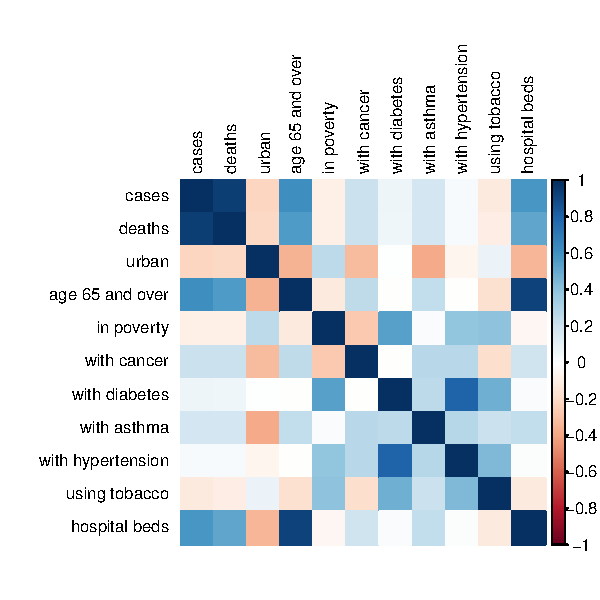
\includegraphics[width=1\linewidth]{draft_files/figure-latex/fig_corr-1} \caption{COVID-19 Mortality and Obesity in Italy}\label{fig:fig_corr}
\end{figure}

\hypertarget{discussion}{%
\section{Discussion}\label{discussion}}


\begin{notes}[Acknowledgements]
\emph{Funding} : C.Z. and L.M.were supported by XXXX.
\end{notes}


\renewcommand\refname{References}

\bibliography{mybibfile.bib}



\end{document}
